\documentclass[prb,preprint]{revtex4-1} 
% The line above defines the type of LaTeX document.
% Note that AJP uses the same style as Phys. Rev. B (prb).

\usepackage{amsmath}  % needed for \tfrac, \bmatrix, etc.
\usepackage{amsfonts} % needed for bold Greek, Fraktur, and blackboard bold
\usepackage{graphicx} % needed for figures

\begin{document}

% Be sure to use the \title, \author, \affiliation, and \abstract macros
% to format your title page.  Don't use lower-level macros to  manually
% adjust the fonts and centering.

\title{Measuring the Verdet Constant in SF-59 Glass}


\author{Liza Mulder}
\email{emulder@smith.edu}
\affiliation{Department of Physics, Smith College, Northampton, MA 01063}


\author{Danika Luntz-Martin}
\email{dluntzma@smith.edu}
\affiliation{Department of Physics, Smith College, Northampton, MA 01063}


\date{\today}



\begin{abstract}

Faraday was the first experimentally observe that light and magnetic field were related. The effect, which bears his name, is a phase shift in the polarization of light due to propagation through a birefringent material in a magnetic field. We observed Faraday Rotation by calculating the polarization of red (650nm) light from a polarized laser propagating through SF-59 glass in various magnetic fields. We determined the Verdet constant, a material specific proportion between magnetic field, length and phase shift. For two different experiments we calculated the Verdet constant for the SF-59 glass rod to be 19.5 $\pm$0.9 $\frac{rad}{Tm}$ and 19.12 $\pm$0.05 $\frac{rad}{Tm}$. These values agree with each other and with the values found by our peer performing similar experiments.

\end{abstract}

\maketitle % title page is now complete


\section{Introduction} % Section titles are automatically converted to all-caps.
% Section numbering is automatic.

Faraday Rotation refers a phenomenon first observed by Faraday in 1945. It was a landmark discovery because it was the first link between light and magnetism.~\cite{teachspin} Faraday discovered that polarized light propagating through certain materials while in a magnetic field experienced a shift in the polarization angle. This effect can be observed in materials which have different refractive indices for left circularly polarized (LCP) light and right circularly polarized (RCP) light when they are in a magnetic field. These materials are called birefringent. Light can be written as the vector sum of LCP and RCP components. When it propagates through the material its components experience different phase shifts leading to a total phase shift in the light's polarization.~\cite{XXX} The magnitude of the phase shift depends on three factors: the strength of the magnetic field, the distance that the light travels in the material and the properties of the material itself. The phase shift for a specific material is given by the Verdet constant ($v_c$) which has units of $\frac{\text{radians}}{\text{tesla\ meter}}$. Thus the equation for total phase shift is $\Delta \theta = v_c B L$.

In this paper, we measure the Verdet constant of SF-59 glass in order to observe the linear relationship expected between phase shift and magnetic field. We performed a second experiment to confirm the value we found for the Verdet constant in our first experiment.

\section{Methods}

Our experimental setup was based off the TeachSpin teaching manual. We used a TeachSpin FRI-A apparatus consisting of a diode laser, a solenoid, a polarizing lens and photodetector. To observe Faraday Rotation and measure the Verdet constant we used a SF-59 glass rod. SF-59 glass is heavy flint glass with a high lead content. The manufacturers dope silicone glass with lead  because the high lead content increases the Verdet constant of the glass, making it easier to observe Faraday Rotation.\cite{opticalglass} We placed the glass rod in the center of the solenoid. The length of our rod was 5 cm shorter than the solenoid so that the magnetic field was approximately constant across the length of the rod and we could neglect the sever drop in magnetic field due to the edges of the solenoid.

\begin{figure}[h!]
\centering
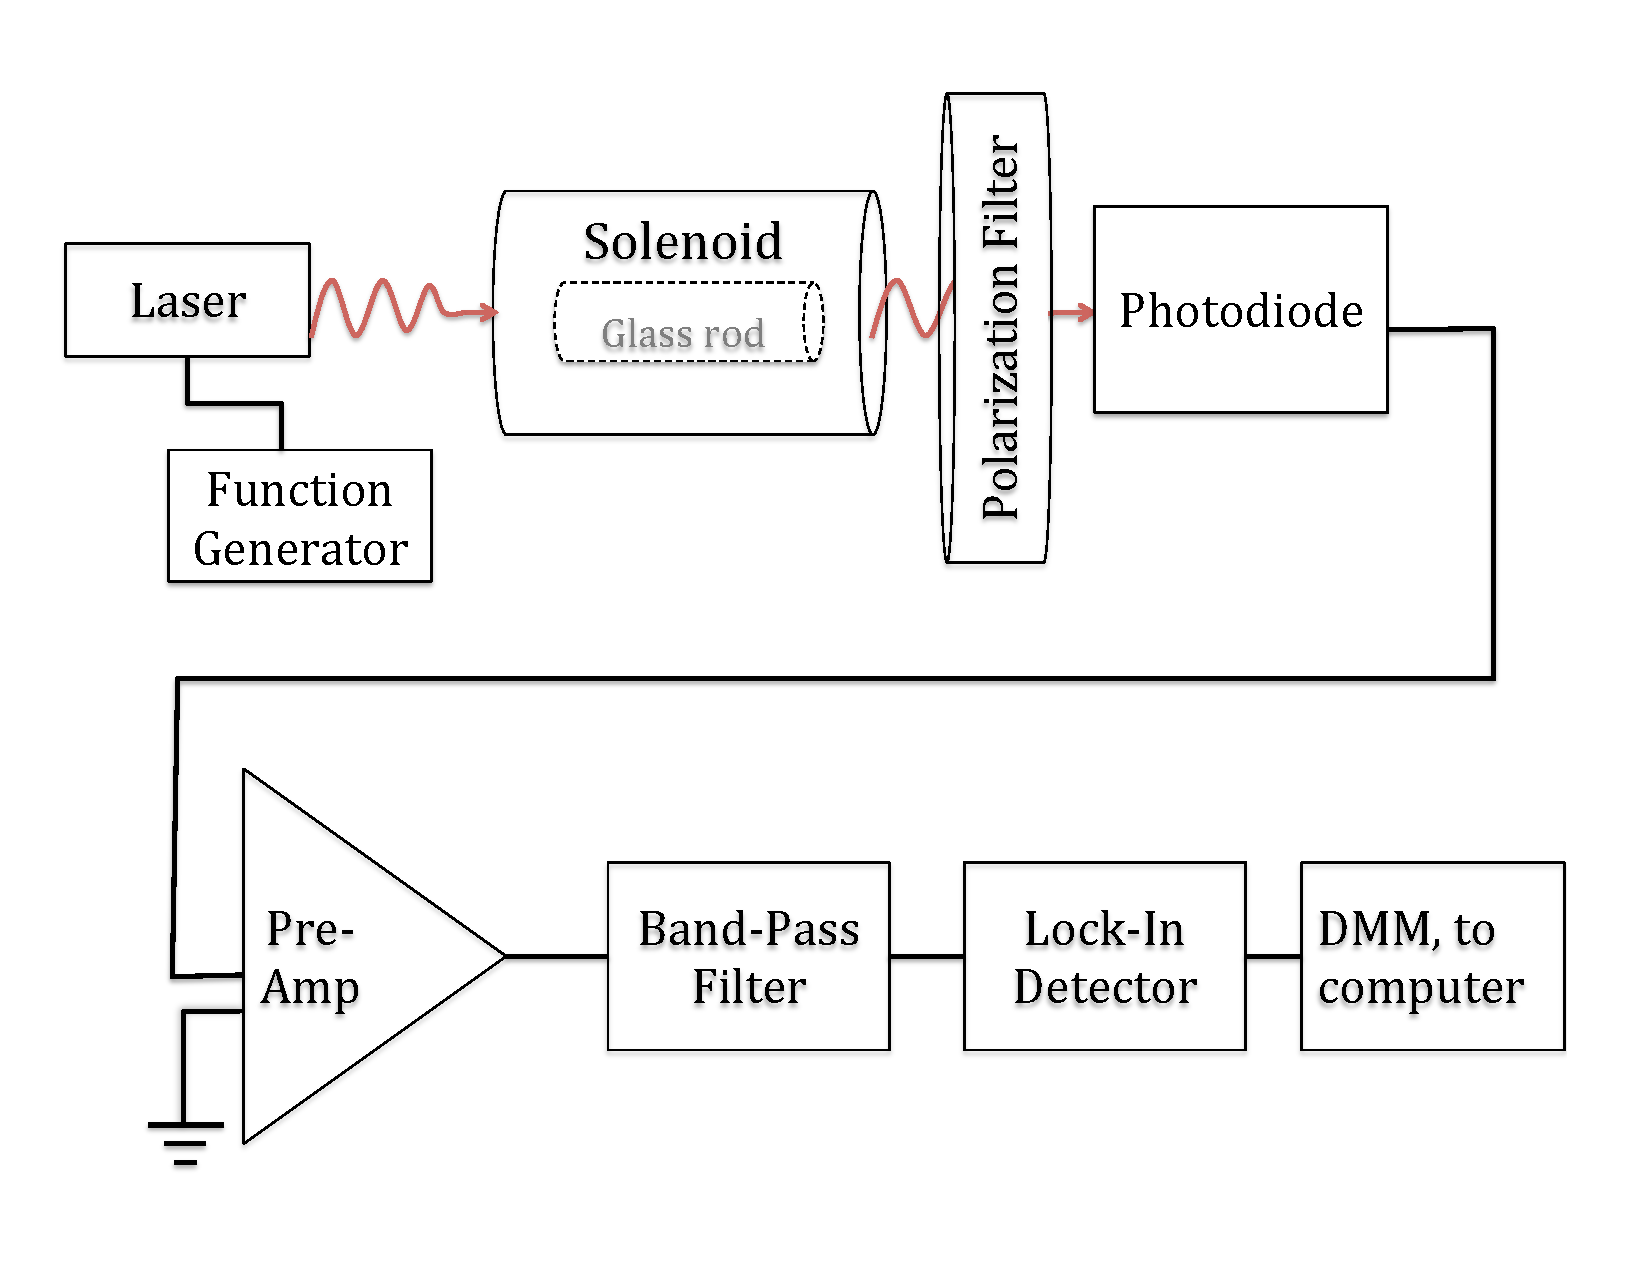
\includegraphics[width=6in]{Faraday_lab_set-up.pdf}
\caption{The set-up of our experiment. The light source was a laser, modulated by a function generator. We sent the beam through a solenoid containing a rod of material, and next a polarization filter. A photodetector at the other end measured the light intensity. This signal went through a  lock-in detector, and from there to the computer.}
\label{set-up}
\end{figure}


Our power source was a Keithley 2230-30-1 Triple Channel DC Power Supply which we used on current control throughout our experiments. We connected the two 3 volt terminals in parallel so that we could obtain a total current of 3 amps through the solenoid. By varying the current through the solenoid we could change the magnetic field through the glass rod. We measured the magnetic field using a TEL-Atomic Inc. Smart Magnetic Sensor for a current of 2A and obtained a field of 21.8mT at the center of solenoid decreasing to 20.5mT at the edges of the glass rod. We took the average of this rage to be our best value and difference between high and low values divided by two to be our uncertainty. To obtain field values for other currents we exploited the linear relationship between magnetic field and current.

We used a Rigol DG1022A function generator to modulate the laser at at frequency of 400Hz. The signal from the photodiode was run through a preamp, a bandpass filter and a lock-in detector. We used lock-in detector to stabilize our measurements and filter out ambient light from the room along with other forms of systematic error.

The output from the lock-in detector was then measured with a Keithley 2100 DMM. To facilitate data collection we used a computer program (helpfully provided by our instructors) called "Keithley DC Incremental Write." The program would record 16 values for voltage, average them and give the result with uncertainty as one data point. 

For our changing theta experiment, we measured the voltage while rotating the polarizing lens. We started with no current through the solenoid and an angle of 90$^{\circ}$ between the polarized laser and the polarizing lens. We found this angle by observing where our intensity and measured voltage were at a minimum. We called this a relative angle of 0$^{\circ}$. We then measured the voltage every 10$^{\circ}$ for a single rotation (360$^{\circ}$). We repeated this measurement for currents of I = 1A, I = 2A and I = 3A.

For our changing field experiment, we set our relative angle to 45$^{\circ}$. We then measured the voltage for currents 0A, $\pm$ 0.5A, $\pm$1A, $\pm$1.5A, $\pm$2A, $\pm$2.5A and $\pm$3A. For each change in current the initial voltage reading would drift as the solenoid heated and resistance changed. We allowed the voltage to stabilize before starting data collect. For this experiment we set the computer program to average over 100 values for each data point.

\section{Results}

From the changing theta experiment, we got 36 data points for each current, i.e. 0A, 1A, 2A, and 3A, shown in Figure ~\ref{V_ThetaRel_Plot}. The red points are the measurements taken without a magnetic field, the orange points were taken with 1A of current passing through the solenoid, the green points with the current at 2A, and the blue points at 3A.  The curve fits are the function $V = A \cos^{2}(\theta + C) - A$, with $A$ held constant at 6.2845 V (obtained from the first curve fit), and $C$ calculated by the curve fit. We are interested in the change in $C$ between curve fits because this gives us the phase shift caused by applying various magnetic fields.

\begin{figure}[h!]
\centering
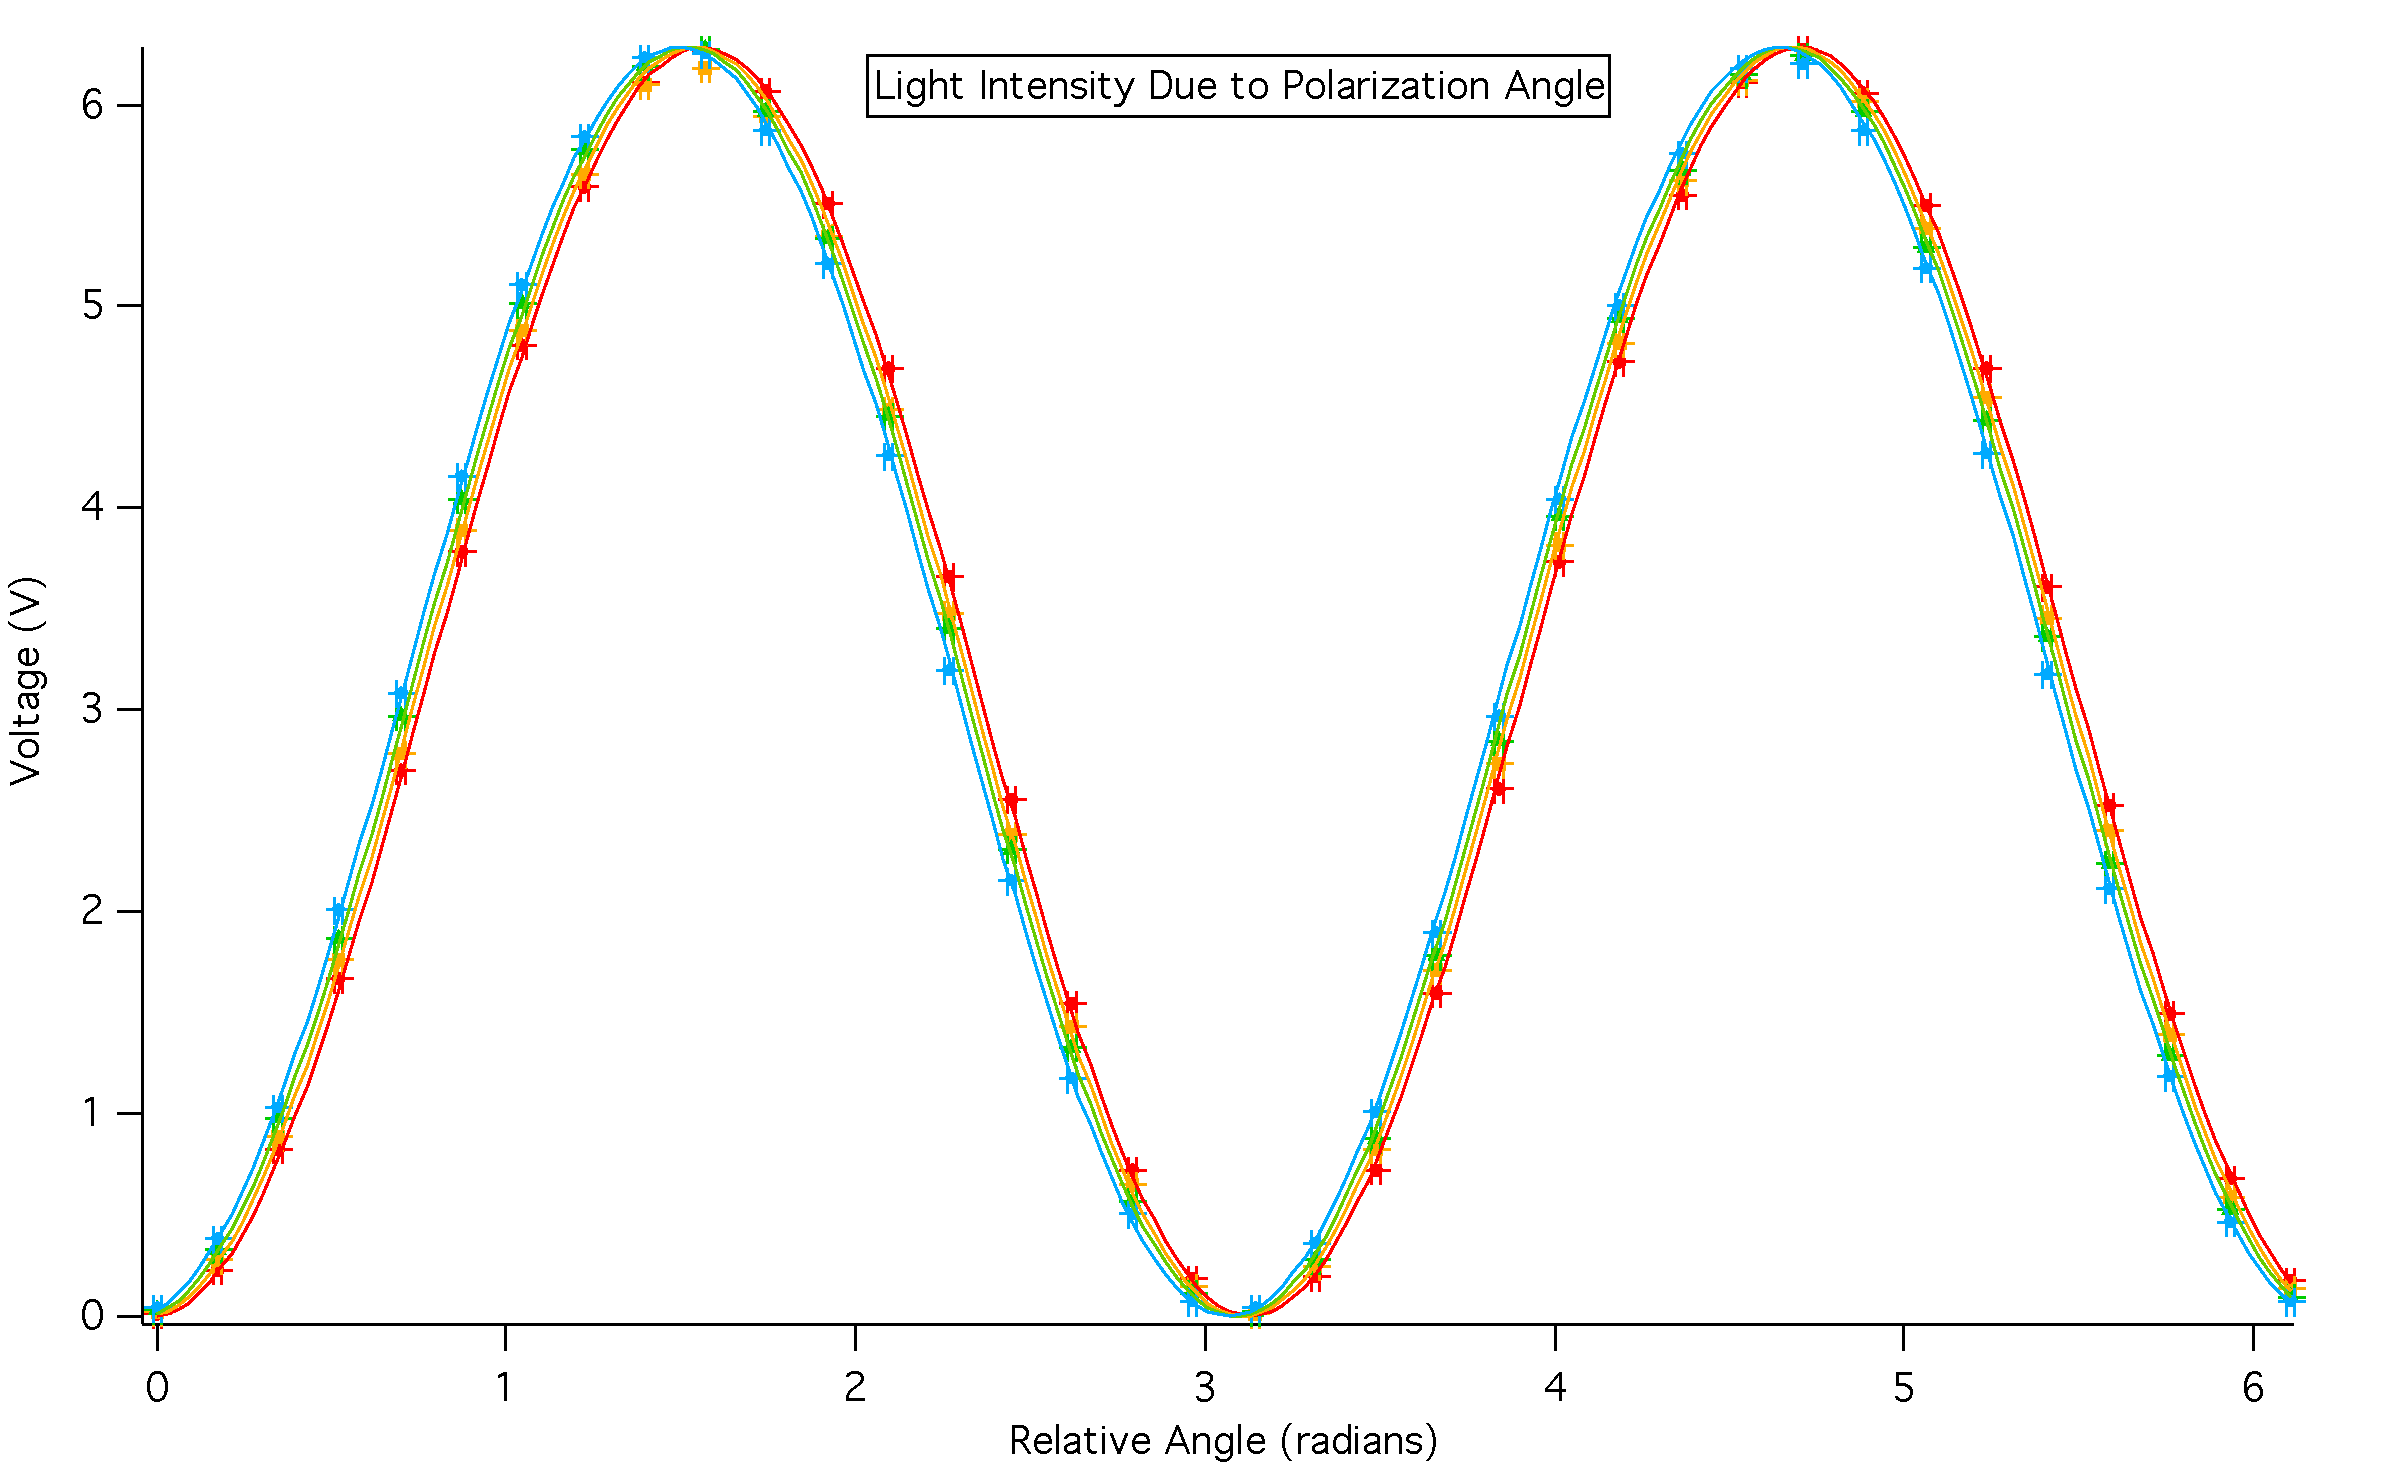
\includegraphics[width=6in]{V_ThetaRel_Plot.pdf}
\caption{Photo-detector voltage (proportional to light intensity) plotted against relative angle from 0 to $\pi$ radians.  The red points are the measurements taken without a current in the solenoid, the orange points were taken with 1A of current, the green points with the current at 2A, and the blue points at 3A.  The curve fits are the function $V = A \cos^{2}(\theta + C) - A$, with $A$ held constant at 6.2845 V (obtained from the first curve fit), and $C$ calculated by the curve fit. }
\label{V_ThetaRel_Plot}
\end{figure}

From the measurements of changing magnetic field, with a constant polarization filter angle, for currents from -3A to 3A in steps of 0.5A, we obtained the results shown in Table ~\ref{V_I_Table}. 

\begin{table}[h!]
\centering
\caption{Voltage readings from the photodetector for various currents applied to the solenoid. }
\begin{ruledtabular}
\begin{tabular}{c c c}
Current (A) & Voltage (V) & Error Voltage (V)\\
\hline	% horizontal line to separate headings from data
-3   & 2.822 & 1.30E-10 \\
-2.5 & 2.887 & 5.47E-10 \\
-2   & 2.951 & 3.72E-10 \\
-1.5 & 3.016 & 3.78E-11 \\
-1   & 3.082 & 8.98E-10 \\
-0.5 & 3.145 & 9.03E-10 \\
0    & 3.211 & 1.18E-09 \\
0.5  & 3.272 & 1.16E-10 \\
1    & 3.338 & 2.05E-09 \\
1.5  & 3.404 & 2.13E-09 \\
2    & 3.468 & 6.96E-10 \\
2.5  & 3.534 & 1.12E-09 \\
3    & 3.599 & 1.05E-09
\end{tabular}
\end{ruledtabular}
\label{V_I_Table}
\end{table}

\section{Analysis}

We analyzed the data from both experiments separately to obtain two estimates for the Verdet Constant.  For the changing theta experiment, we used IgorPro to fit the function $V = A \cos ^2 (\theta + C) - A$ to the data in Figure ~\ref{V_ThetaRel_Plot}.  We then calculated the magnetic field from the applied current and our measurements for field at 2A, and the phase shift from the difference between the c-values of the curve fits.  The results are in Table ~\ref{B*L_PhaseShift_Table}.  

\begin{table}[h!]
\centering
\caption{Curve fit data and calculated phase shifts for changing angle experiment, with magnetic fields calculated from the applied currents.}
\begin{ruledtabular}
\begin{tabular}{c c c c c c c}
I (A) & BL (mT cm) & $\delta$BL (mT cm) & C (rad)& $\delta$C (rad) & $\Delta \theta$ (rad) & $\delta \Delta \theta$ (rad)\\
\hline	% horizontal line to separate headings from data
0 &  0  & 0 &  0.0088553 & 0.001 & 0 & 0.002    \\
1 & 108 & 4  & 0.030849  & 0.0014 & 0.022  & 0.0024 \\
2 & 215 & 8 & 0.049599  & 0.0013 & 0.0407 & 0.0023  \\
3 & 323 & 12 & 0.072754  & 0.0015 & 0.0639 & 0.0025 
\end{tabular}
\end{ruledtabular}
\label{B*L_PhaseShift_Table}
\end{table}

We then plotted the phase shift versus the magnetic field multiplied by the length of our rod, which gave us Figure ~\ref{PhaseShift_B*L_Plot}. From the theory we know that $\Delta \theta = v_c B L$ therefore we would expect our data to be linear and the Verdet constant to be the slope.

\begin{figure}[h!]
\centering
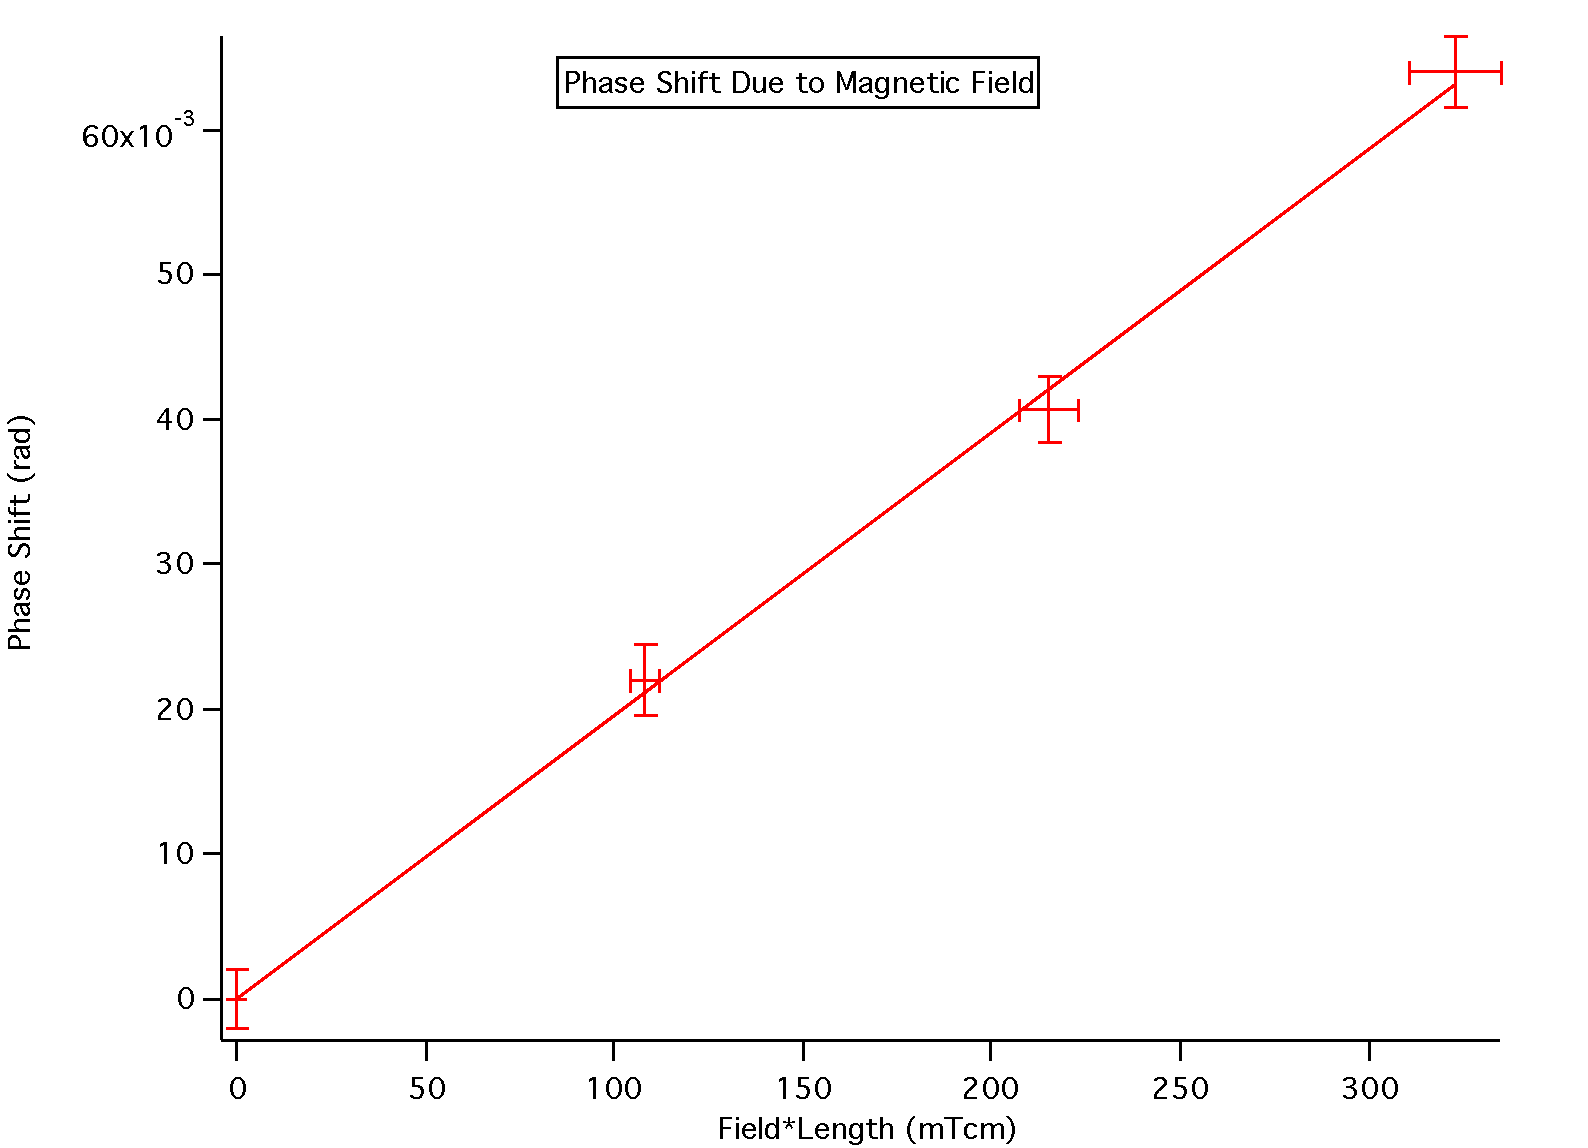
\includegraphics[width=5in]{PhaseShift_B-L_Plot.pdf}
\caption{A plot of Table \ref{B*L_PhaseShift_Table}, applied magnetic field (times length of the refracting material) versus the resulting phase shift in the polarization of the laser beam. The slope of a linear curve fit of this plot gives a value for the Verdet constant of the material. }
\label{PhaseShift_B*L_Plot}
\end{figure}

From the linear fit of our plot we obtained a slope $19.5 \pm0.9 \frac{1}{Tm}$.

To get the Verdet constant from our changing field experiment, we first calculated the values of magnetic field times length for currents from -3A to 3A in steps of 0.5As. As before we calculated the field from our measured field for 2A and the linear relationship between field and current. The results are in Table ~\ref{V_B*L_Table}. 

\begin{table}[h!]
\centering
\caption{The fields due to the currents in table ~\ref{V_I_Table} applied to our solenoid, with the resulting voltage measured by the photodetector. }
\begin{ruledtabular}
\begin{tabular}{c c c c}
Magnetic Field * Length (mT*cm) & Error B*L (mT*cm) & Voltage (V) & Error Voltage (V)\\
\hline	% horizontal line to separate headings from data
-323 & 12 & 2.822 & 1.30E-10 \\
-269 & 10 & 2.887 & 5.47E-10 \\
-215 & 8  & 2.951 & 3.72E-10 \\
-161 & 6  & 3.016 & 3.78E-11 \\
-108 & 4  & 3.082 & 8.98E-10 \\
-54  & 2  & 3.145 & 9.03E-10 \\
0    & 0  & 3.211 & 1.18E-09 \\
54   & 2  & 3.272 & 1.16E-10 \\
108  & 4  & 3.338 & 2.05E-09 \\
161  & 6  & 3.404 & 2.13E-09 \\
215  & 8  & 3.468 & 6.96E-10 \\
269  & 10 & 3.534 & 1.12E-09 \\
323  & 12 & 3.599 & 1.05E-09
\end{tabular}
\end{ruledtabular}
\label{V_B*L_Table}
\end{table}

We plotted the results of Table ~\ref{V_B*L_Table} in Figure ~\ref{V_B*L_Plot}. From the slope of the linear fit of this plot we got $\frac{\delta V}{\delta BL}$

\begin{figure}[h!]
\centering
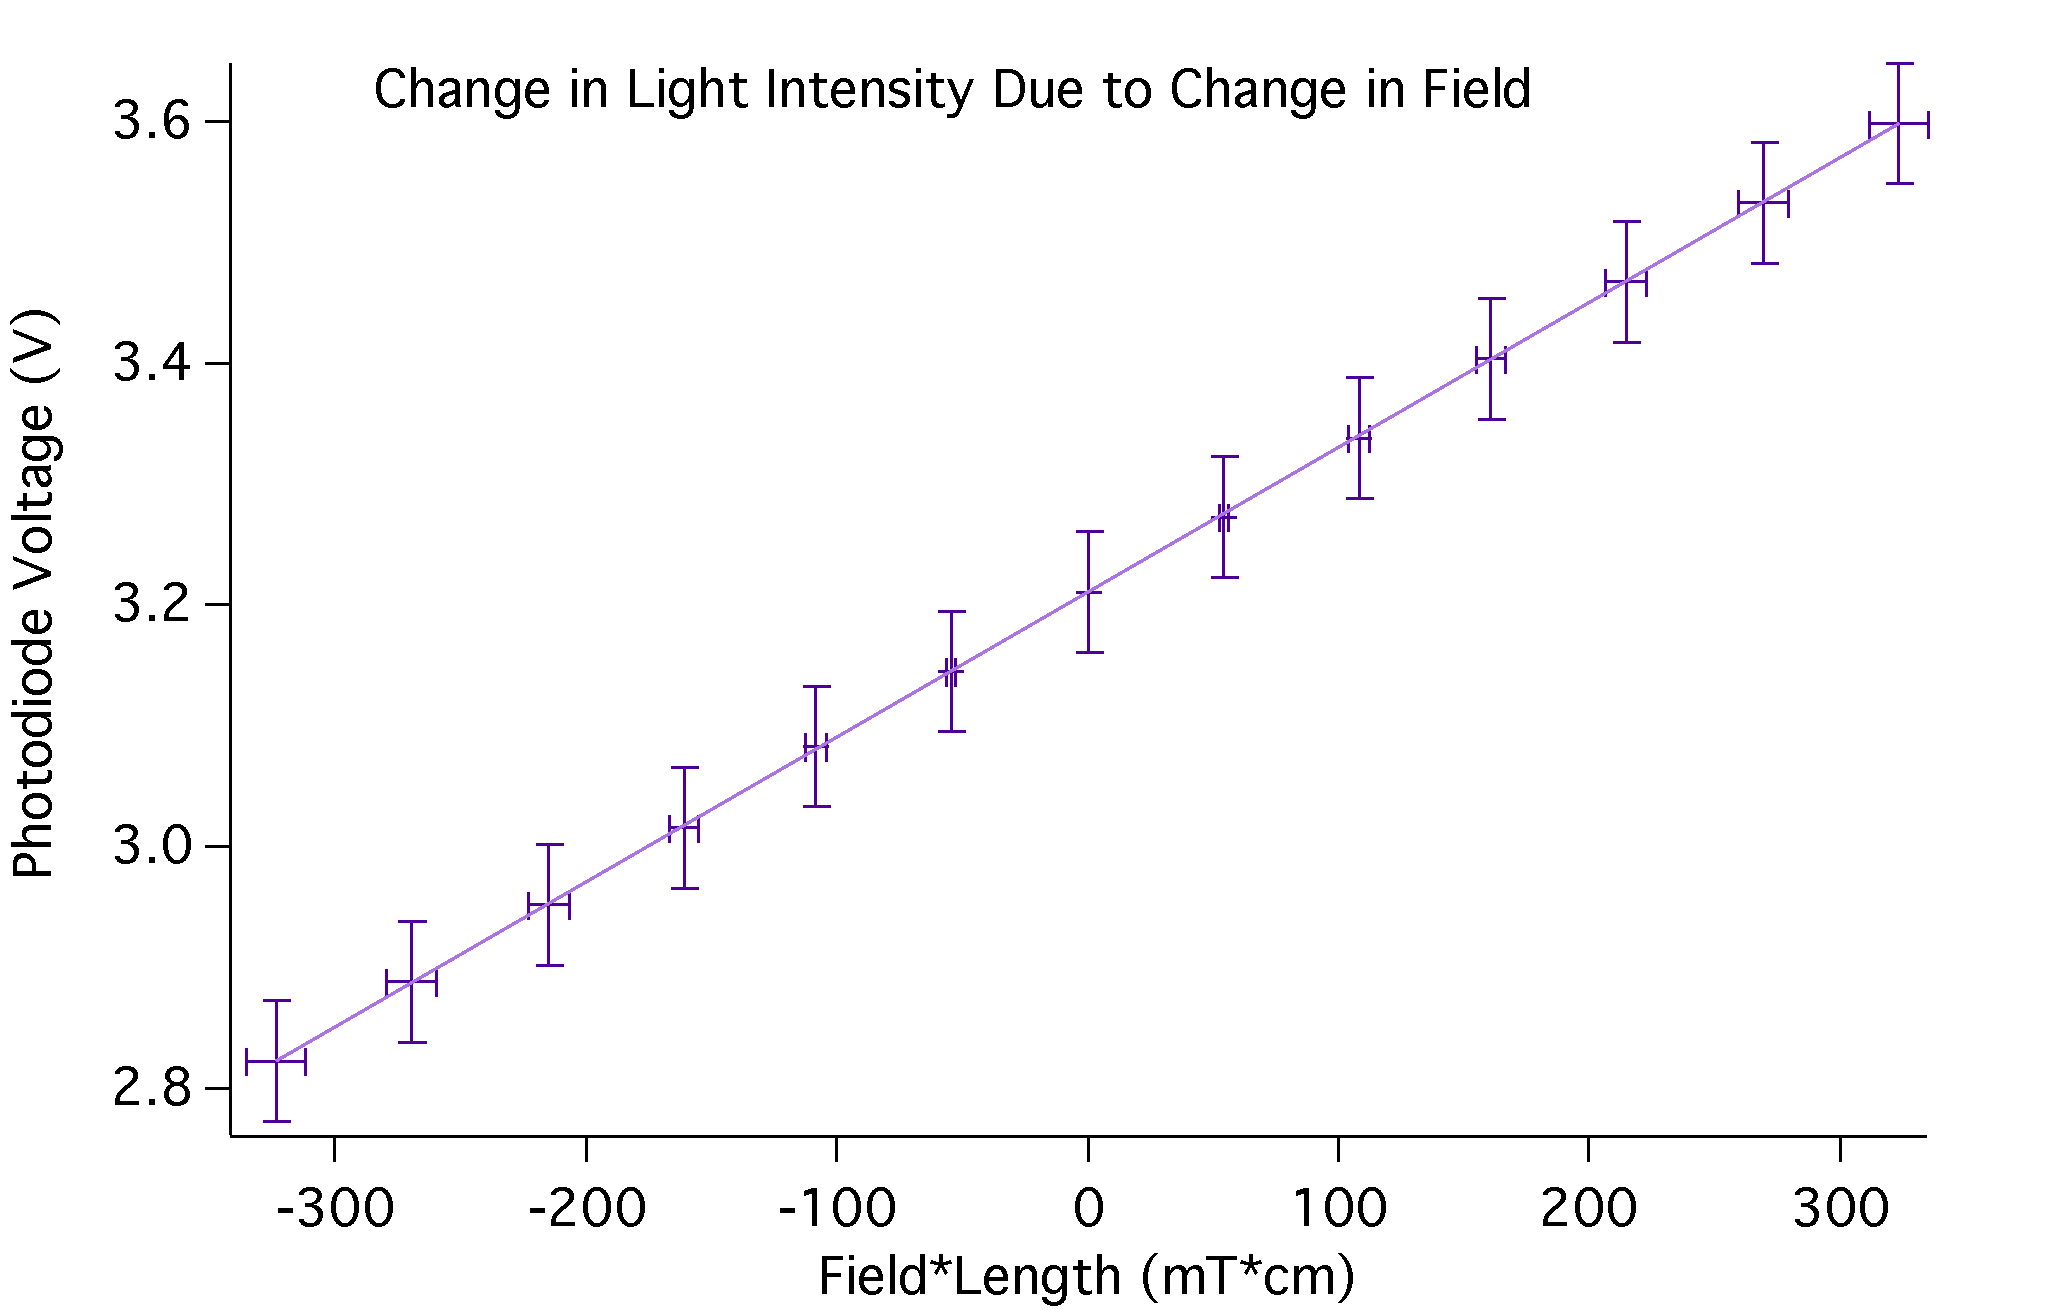
\includegraphics[width=5in]{V_B-L_Plot.pdf}
\caption{A plot of Table \ref{V_B*L_Table}, the applied magnetic field (times the length of the refracting material) versus the voltage measured by the photodetector for that field. The slope of a linear curve fit to this plot can be used to calculate the Verdet constant of the material. }
\label{V_B*L_Plot}
\end{figure}

Since, as shown above $v_c = \frac{\delta \theta}{\delta BL}$, we can use the chain rule for derivatives and get: 
\\
$\frac{\delta V}{\delta BL} = \frac{\delta V}{\delta \theta} \frac{\delta \theta}{\delta BL} = \frac{\delta V}{\delta \theta} v_c$.  
\\
Therefore $v_c = \frac{\frac{\delta V}{\delta BL}}{\frac{\delta V}{\delta \theta}}$.
\\
From Figure ~\ref{V_B*L_Plot} we got $\frac{\delta V}{\delta BL} = 0.0012018 \pm 1.8 \times 10^{-6}$. To get $\frac{\delta V}{\delta \theta}$, we took the derivative of the function $V = A \cos^{2}(\theta) - A$ at $\theta = \pi/4$ and obtained $\frac{\delta V}{\delta \theta} = -A$, and from the fit to the zero field data in Figure ~\ref{V_ThetaRel_Plot}, $-A = 6.285 \pm 0.008 V$.  

Dividing these two results, we get $v_c = \frac{\frac{\delta V}{\delta BL}}{\frac{\delta V}{\delta \theta}} = 19.12 \pm 0.05 \frac{1}{Tm}$.  

%\begin{table}[h!]
%\centering
%\caption{C values taken from the curve fits to Figure ~\ref{V_ThetaRel_Plot}}
%\begin{ruledtabular}
%\begin{tabular}{c c c}
%Current (A) & C value from curve fit (rad) & Error C value (rad)\\
%\hline	% horizontal line to separate headings from data
%0 & 0.0088553 & 0.001  \\
%1 & 0.030849  & 0.0014 \\
%2 & 0.049599  & 0.0013 \\
%3 & 0.072754  & 0.0015
%\end{tabular}
%\end{ruledtabular}
%\label{I_cValue_Table}
%\end{table}




\section{Discussion}

All of our data fit the expected relationships. In Figure ~\ref{V_ThetaRel_Plot} the intensity of the light, given by voltage from the photodetector, showed a $\cos^2\theta$ relationship with relative angle between the laser and the polarizing filter as was expected. For the changing theta experiment the relationship between phase shift and magnetic field had a constant, positive slope, Figure ~\ref{PhaseShift_B*L_Plot}, which is reassuring since slope should be the Verdet constant, a constant positive value.  For the changing field experiment we expect intensity to depend linearly on field because a change in field causes a proportional change in phase shift and the relationship between intensity, i.e. voltage, and phase shift to be linear for small changes in phase. The values that we obtained for the Verdet constant from both experiments agreed with each other within uncertainty. 

The biggest sources of error in our experiments came from our measurement of the magnetic field and the imprecision of our angle measurement on the polarizing filter. To decrease error in future experiments we would suggest using a more accurate magnetic field sensor and to measure the magnetic field for all currents used in the experiment. 


\begin{thebibliography}{3}

\bibitem{melissanos} Adrian C. Melissanos and Jim Napoitano, \textit{Experiments in Modern Physics} 2nd edition (Academic Press, Boston, 2003)

\bibitem{teachspin} Jonathan F. Reichert, \textit{Faraday Rotation: Instructor's Guide to TeachSpin's FRI-A Apparatus}

\bibitem{opticalglass} Hans Bach and Norbert Neuroth, \textit{The Properties of Optical Glass} 2nd edition (Springer Science and Business Media, Mainz, Germany,1998)

\end{thebibliography}
\end{document}
